\documentclass[a4paper,12pt]{article} % добавить leqno в [] для нумерации слева
\usepackage[a4paper,top=1.3cm,bottom=2cm,left=1.5cm,right=1.5cm,marginparwidth=0.75cm]{geometry}
%%% Работа с русским языком
\usepackage{cmap}					% поиск в PDF
\usepackage[warn]{mathtext} 		% русские буквы в фомулах
\usepackage[T2A]{fontenc}			% кодировка
\usepackage[utf8]{inputenc}			% кодировка исходного текста
\usepackage[english,russian]{babel}	% локализация и переносы
\usepackage{physics}
\usepackage{multirow}
\usepackage{siunitx}

%%% Нормальное размещение таблиц (писать [H] в окружении таблицы)
\usepackage{float}
\restylefloat{table}

\usepackage{graphicx}

\usepackage{caption}
\usepackage{subcaption}

\usepackage{wrapfig}
\usepackage{tabularx}

\usepackage{hyperref}
\usepackage[rgb]{xcolor}
\hypersetup{
	colorlinks=true,urlcolor=blue
}

%%% Дополнительная работа с математикой
\usepackage{amsmath,amsfonts,amssymb,amsthm,mathtools} % AMS
\usepackage{icomma} % "Умная" запятая: $0,2$ --- число, $0, 2$ --- перечисление

%% Номера формул
%\mathtoolsset{showonlyrefs=true} % Показывать номера только у тех формул, на которые есть \eqref{} в тексте.

%% Шрифты
\usepackage{euscript}	 % Шрифт Евклид
\usepackage{mathrsfs} % Красивый матшрифт
\usepackage{pgfplots}
\pgfplotsset{compat=1.9}

%% Свои команды
\DeclareMathOperator{\sgn}{\mathop{sgn}}

%% Перенос знаков в формулах (по Львовскому)
\newcommand*{\hm}[1]{#1\nobreak\discretionary{}
	{\hbox{$\mathsurround=0pt #1$}}{}}

\date{\today}

\begin{document}

\begin{titlepage}
	\begin{center}
		{\large МОСКОВСКИЙ ФИЗИКО-ТЕХНИЧЕСКИЙ ИНСТИТУТ (НАЦИОНАЛЬНЫЙ ИССЛЕДОВАТЕЛЬСКИЙ УНИВЕРСИТЕТ)}
	\end{center}
	\begin{center}
		{\large Физтех-школа прикладной математики и информатики}
	\end{center}
	
	
	\vspace{4.5cm}
	{\huge
		\begin{center}
			{\bf Отчёт о выполнении лабораторной работы 4.5.3}\\
			Сканирующий интерферометр
		\end{center}
	}
	\vspace{1cm}
	\begin{center}
		{\large Соболевский Федор Александрович \\
                    Старокожко Иван Георгиевич \\
			\vspace{0.2cm}
			Б05-111}
	\end{center}
	\vspace{8cm}
	\begin{center}
		  Апрель 2023
	\end{center}
\end{titlepage}

\section{Аннотация}
В данной работе изучены устройство и работа гелий-неонового лазера непрерывного действия и сканирующего интерферометра Фабри-Перо. С помощью интерферометра изучен спектральный состав лазера и его количественные характеристики. По полученным осциллограммам оценены газокинетические и спектральные характеристики лазера и разрешающая способность интерферометра.

\section{Теоретически сведения}
\subsection*{Лазер и его спектральный состав}
\textbf{Лазер} есть источник квазимонохроматического и узконаправленного высококогерентного потока излучения, работающий за счёт квантово-механического эффекта вынужденного (индуцированного) излучения. В гелий-неоновом лазере резонатором является система из двух зеркал с высоким коэффициентом отражения~---\textbf{интерферометр Фабри-Перо}~--- и активная среда, состоящая из гелия и неона.

\begin{figure}[h]
    \centering
    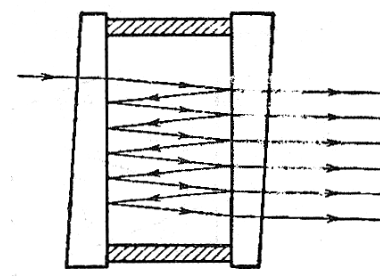
\includegraphics[width=0.3\textwidth]{interfp.png}
    \caption{Принцип работы интерферометра Фабри-Перо}
    \label{fig:interfp}
\end{figure}
Схематично принцип работы интерферометра Фабри-Перо изображён на рис. \ref{fig:interfp}. Между зеркалами вдоль оси интерферометра многократно отражается свет, при этом максимальным усилением в силу интерференции обладают волны, для которых набег фазы при полном обходе резонатора кратен $2 \pi$, откуда
\begin{equation}\label{modeCond}
    2L = m\lambda,\quad m\in\mathbb{N},
\end{equation}
где $L$~--- длина резонатора.Тогда разность соседних усиливаемых частот излучения есть
\begin{equation}\label{modeDiff}
    \nu_{m+1} - \nu_m = \frac{c}{2L}.
\end{equation}
\begin{figure}[h]
    \centering
    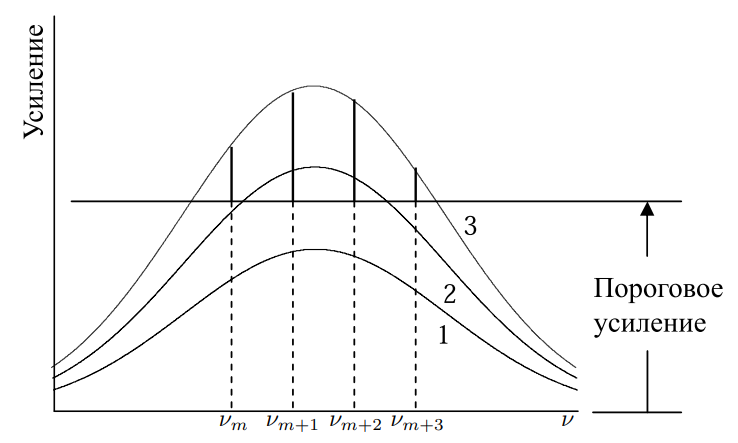
\includegraphics[width=0.7\textwidth]{modeCount.png}
    \caption{Зависимость количества мод от усиления лазера}
    \label{fig:modeCount}
\end{figure}
Соответственно, лазер генерирует отдельные типы колебаний, называемые модами, удовлетворяющие условию \eqref{modeCond}. Количество мод определяется усилением лазера (см. рис. \ref{fig:modeCount}) и шириной спектра генерации, которая, в свою очередь, обусловена \textbf{эффектом Доплера}~--- явлением изменения частоты генерируемого излучения вследствие хаотического теплового движения излучающих атомов. Частота излучения движущегося источника сдвинута относительно неподвижного источника; в нерелятивистском случае
\begin{equation}\label{dope}
    \frac{\Delta\omega_D}{\omega} \sim \frac{v}{c}\cos\alpha,
\end{equation}
где $\Delta\omega_D$~--- смещение частоты излучения относительно излучения источника, $\alpha$~--- угол между вектором скорости и направлением на наблюдателя. В предположении, что $\cos\alpha$ случайно меняется в пределах от -1 до 1, усреднением получим приближённую формулу для ширины доплеровского контура:
\begin{equation}\label{DoppWidth}
    \Delta\omega_D = \frac{\omega}{c}\sqrt{\frac{8kT}{\pi m}}.
\end{equation}
Приведём более точную формулу из спектрометрии:
\begin{equation}
    \label{cool_DoppWidth}
    \Delta\nu_D = \sqrt{\ln 2}\cdot\frac{\nu_{max}}{c}\sqrt{\frac{2kT}{m}}, 
\end{equation}
где $\nu_\text{max}$~--- частота излучения лазера.
В данной работе мы предполагаем, что ширина спектра излучения определяется преимущественно эффектом Доплера. В действительности же она также зависит от случайного шума и потерь энергии в системе, поэтому в ходе работы, помимо прочего, проверяется, насколько верно данное приближение.

\subsection*{Сканирующий интерферометр}
\begin{figure}[h]
    \centering
    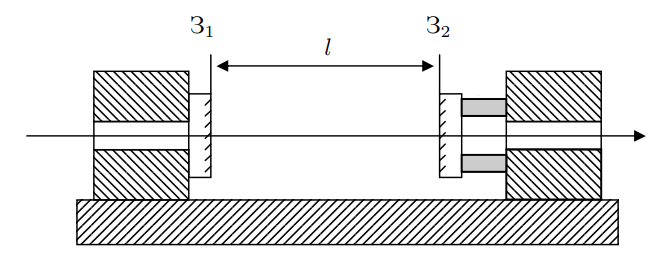
\includegraphics[width=0.7\textwidth]{scanner.png}
    \caption{Схема устройства сканирующего интерферометра}
    \label{fig:scanner}
\end{figure}
В данной работе для наблюдения спектра излучения лазера использовался \textbf{сканирующий интерферометр}~--- интерферометр Фабри-Перо с быстро изменяющимся во времени расстоянием между отражающими пластинами. Схематично эта система изображена на рис. \ref{fig:scanner}. Для интерферометра выполняются соотношения, аналогичные \eqref{modeCond}, \eqref{modeDiff}, определяющие длину волны излучения, полностью проходящего через прибор, т.\,е. его \textit{собственные моды}. Разность частот собственных мод интерферометра называется \textit{дисперсионной областью} и выражается в единицах длины волны как
\begin{equation}
    \Delta\lambda = \frac{\lambda}{m} = \frac{\lambda^2}{2l}.
\end{equation}
Здесь $l$~--- расстояние между пластинами интерферометра. В данной работе интерферометр используется как оптический прибор высокой разрешающей силы. Разрешающая способность $R$ определяется как
\begin{equation}
    \label{eq:R}
    R = \frac{\lambda}{\delta\lambda},
\end{equation}
где $\delta\lambda$~--- минимальная разность длин волн, разрешаемая прибором вблизи длины волны $\lambda$. В случае интерферометра Фабри—Перо две линии считаются разрешимыми, если расстояние между максимумами их контуров равно или превышает ширину контура по уровню 0,5. Разрешающая способность интерферометра Фабри—Перо зависит от длины интерферометра $l$ и коэффициента отражения зеркал $r$:
\begin{equation} \label{eq:R_r}
    R = \frac{2\pi l}{\lambda(1-r)}.
\end{equation}
В сканирующем интерферометре величина $l$ периодически меняется, что обеспечивает прохождение через прибор разных длин волн лазерного излучения в разные промежутки времени и в конечном счёте образует периодический световой сигнал, представляющий собой спектр излучения лазера. Если амплитуда изменения $l$ больше половины длины волны, то спектральная картина после смещения на $\lambda/2$ начинает повторяться. Это проиллюстрировано на рис. \ref{fig:oscillog}.
\begin{figure}
    \centering
    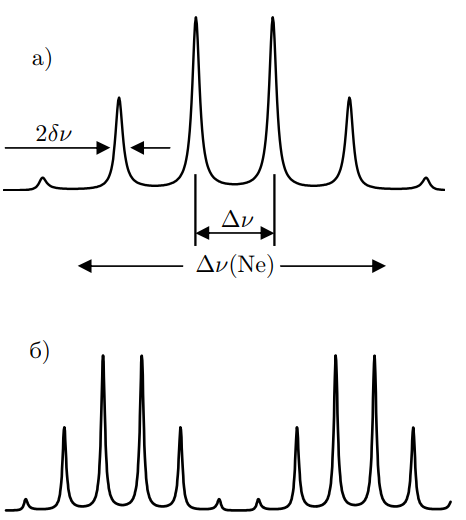
\includegraphics[width=0.45\textwidth]{oscillog.png}
    \caption{Характерные осциллограммы: а) при небольшой амплитуде
колебаний зеркала ($\leq\lambda$/2), б) при амплитуде колебаний, превышающей $\lambda$/2}
    \label{fig:oscillog}
\end{figure}

\section{Экспериментальная установка}
\begin{figure}[h]
    \centering
    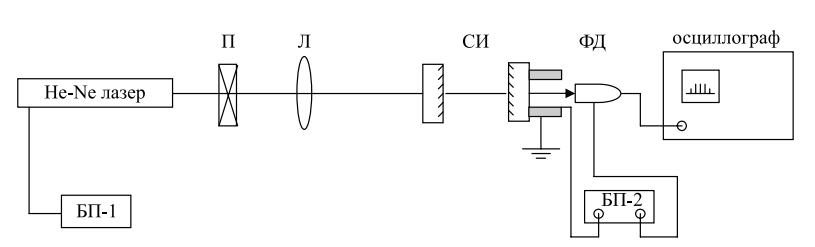
\includegraphics[width=0.8\textwidth]{setup.png}
    \caption{Схема экспериментальной установки}
    \label{fig:setup}
\end{figure}
Схема экспериментальной установки изображена на рис. \ref{fig:setup}.
Излучение He–Ne-лазера проходит через поляризационную развязку Р и линзу Л и поступает на вход сканирующего интерферометра (СИ). Поляризационная развязка предотвращает попадание в лазер излучения, отразившегося от элементов 
 оптического тракта. Это излучение может существенно повлиять на работу лазера и даже привести к срыву генерации. Развязка состоит из поляроида и пластинки $\lambda$/4, главные направления которой установлены под углом 45$^\text{o}$ по отношению к разрешённому направлению поляроида. После развязки П свет приобретает циркулярную поляризацию (например, по правому кругу). При отражении от передней поверхности линзы, от зеркала сканирующего интерферометра и т.п. свет распространяется в обратном направлении в виде левополяризованной волны. Такая волна, пройдя через пластинку $\lambda$/4, вновь приобретает линейную поляризацию. Однако направление колебаний в этой волне оказывается перпендикулярным направлению разрешённых колебаний поляроида, поэтому до лазера отражённая волна не доходит. 

Линза Л служит для уменьшения расходимости пучка, поступающего на вход сканирующего интерферометра. Линза снабжена поперечными и продольными салазками для юстировки прибора на максимум сигнала. Излучение, прошедшее сквозь сканирующий интерферометр, поступает на фотодиод ФД. Напряжение с фотодиода через усилитель подаётся на вертикальный вход электронного осциллографа ЭО.

Лазер питается от блока питания БП-1, фотодиод и усилитель~---
от БП-2. Напряжение на пьезоэлемент сканирующего интерферометра
подаётся с блока питания БП-2 и регулируется ручкой 1.

\section{Ход работы, результаты}\label{sectionref}

\subsection{Определение периода решёток по их пространственному спектру}
Для первого метода было измерено расстояние между дифракционными максимумами пространственного спектра. Расстояние от экрана до решетки~--- $L = 1282 \text{ мм}$, длина волны лазера здесь и далее~--- $\lambda = 532 \text{ нм}$. Здесь и далее систематическая погрешность измерения длин с помощью линейки равна $\Delta_L = 1$ мм, с помощью нониусного винта линзы~--- $\Delta_x = 0,1$ мм. 

Выразив $\sin\theta_n$ через расстояние до экрана и до $n$-ого максимума, получаем следующее выражение для периода решетки:
\[
d \sin \theta = m \lambda \Longrightarrow d = \frac{L \lambda \cdot N}{X_N}.
\]
Измерения данным методом были проведены для всех двумерных решёток (1-5). Результаты представлены в таблице \ref{tab1}. Погрешность в данном эксперименте можно считать зависящей в основном от систематической. 

\begin{table}[!ht]
    \centering
    \begin{tabular}{|l|l|l|l|l|}
    \hline
        № & $N$ & $X_N$, мм & $x_0$, мм & $d$, см \\ \hline
        1 & 6 & 204 & 34,0 & 0,020$\pm0,003$ \\ \hline
        2 & 4 & 81 & 20,3 & 0,034$\pm0,005$ \\ \hline
        3 & 13 & 148 & 11,4 & 0,0600$\pm0,003$ \\ \hline
        4 & 15 & 90 & 6,0 & 0,114$\pm0,004$ \\ \hline
        5 & 35 & 150 & 4,3 & 0,159$\pm0,006$ \\ \hline
    \end{tabular}
    \caption{Результаты измерения периодов решёток по пространственному спектру}
    \label{tab1}
\end{table}

\subsection{Определение периода решеток по изображению, увеличенному с помощью линзы}
Для второго метода в схему была добавлена собирающая линза, создающая увеличенное изображение на экране. При помощи проволчки, то есть непериодического объекта, найдено первое изображение. Размеры изображений могут быть найдены из формулы увеличения:
\[
d = D \frac ab,
\]
где $a$~--- расстояние до линзы, $b$~--- до экрана. Результаты измерения периодов представлены в таблице \ref{tab2}. Здесь вклад в погрешность вносит также усреднение при расчёте $D$. Также отметим, что в силу мелкости картины не удалось измерить период данным способом для решёток 1 и 2.
\begin{table}[!ht]
    \centering
    \begin{tabular}{|l|l|l|l|}
    \hline
        № & $X_N$, мм & $x_0$, мм & $d$, см \\ \hline
        3 & 51 & 1,8 & 0,089$\pm0,012$ \\ \hline
        4 & 49 & 2,9 & 0,140$\pm0,018$ \\ \hline
        5 & 41 & 3,2 & 0,153$\pm0,022$ \\ \hline
    \end{tabular}
    \caption{Результаты измерения периодов решёток по геометрическому изображению}
    \label{tab2}
\end{table}

\subsection{Исследование эффекта саморепродукции с помощью сеток}
Далее для каждой решетки измерена зависимость координаты саморепродуцированного изображения от его номера. По коэффициенту зависимости можно найти период решетки:
\[
d = \sqrt{ \frac{k\lambda}{2} }
\]
Результаты представлены в таблице \ref{tab3}. Здесь в погрешность измерений входит случайная ошибка метода наилучшей прямой. Графики зависимостей изображены на рис.~\ref{fig:plot} (там же изображены графики для решёток миры, см. далее).

\begin{table}[!ht]
    \centering
    \begin{tabular}{|l|l|l|l|l|l|l|l|l|l|}
    \hline
        № & 0 & 1 & 2 & 3 & 4 & 5 & 6 & k, мм & d, см \\ \hline
        3 & 37,45 & 41,2 & 44,1 & 48,2 & 50,7 & 54,95 & 56,3 & 3,24 & 0,093$\pm0,011$ \\ \hline
        4 & 37,2 & 42,05 & 50,65 & 57,375 & 64,1 & - & - & 6,91 & 0,136$\pm0,016$ \\ \hline
        5 & 37,6 & 48,45 & - & - & - & - & - & 10,85 & 0,170$\pm0,035$ \\ \hline
    \end{tabular}
    \caption{Результаты измерения периодов решёток по репродукции}
    \label{tab3}
\end{table}

\begin{figure}[H]
    \centering
    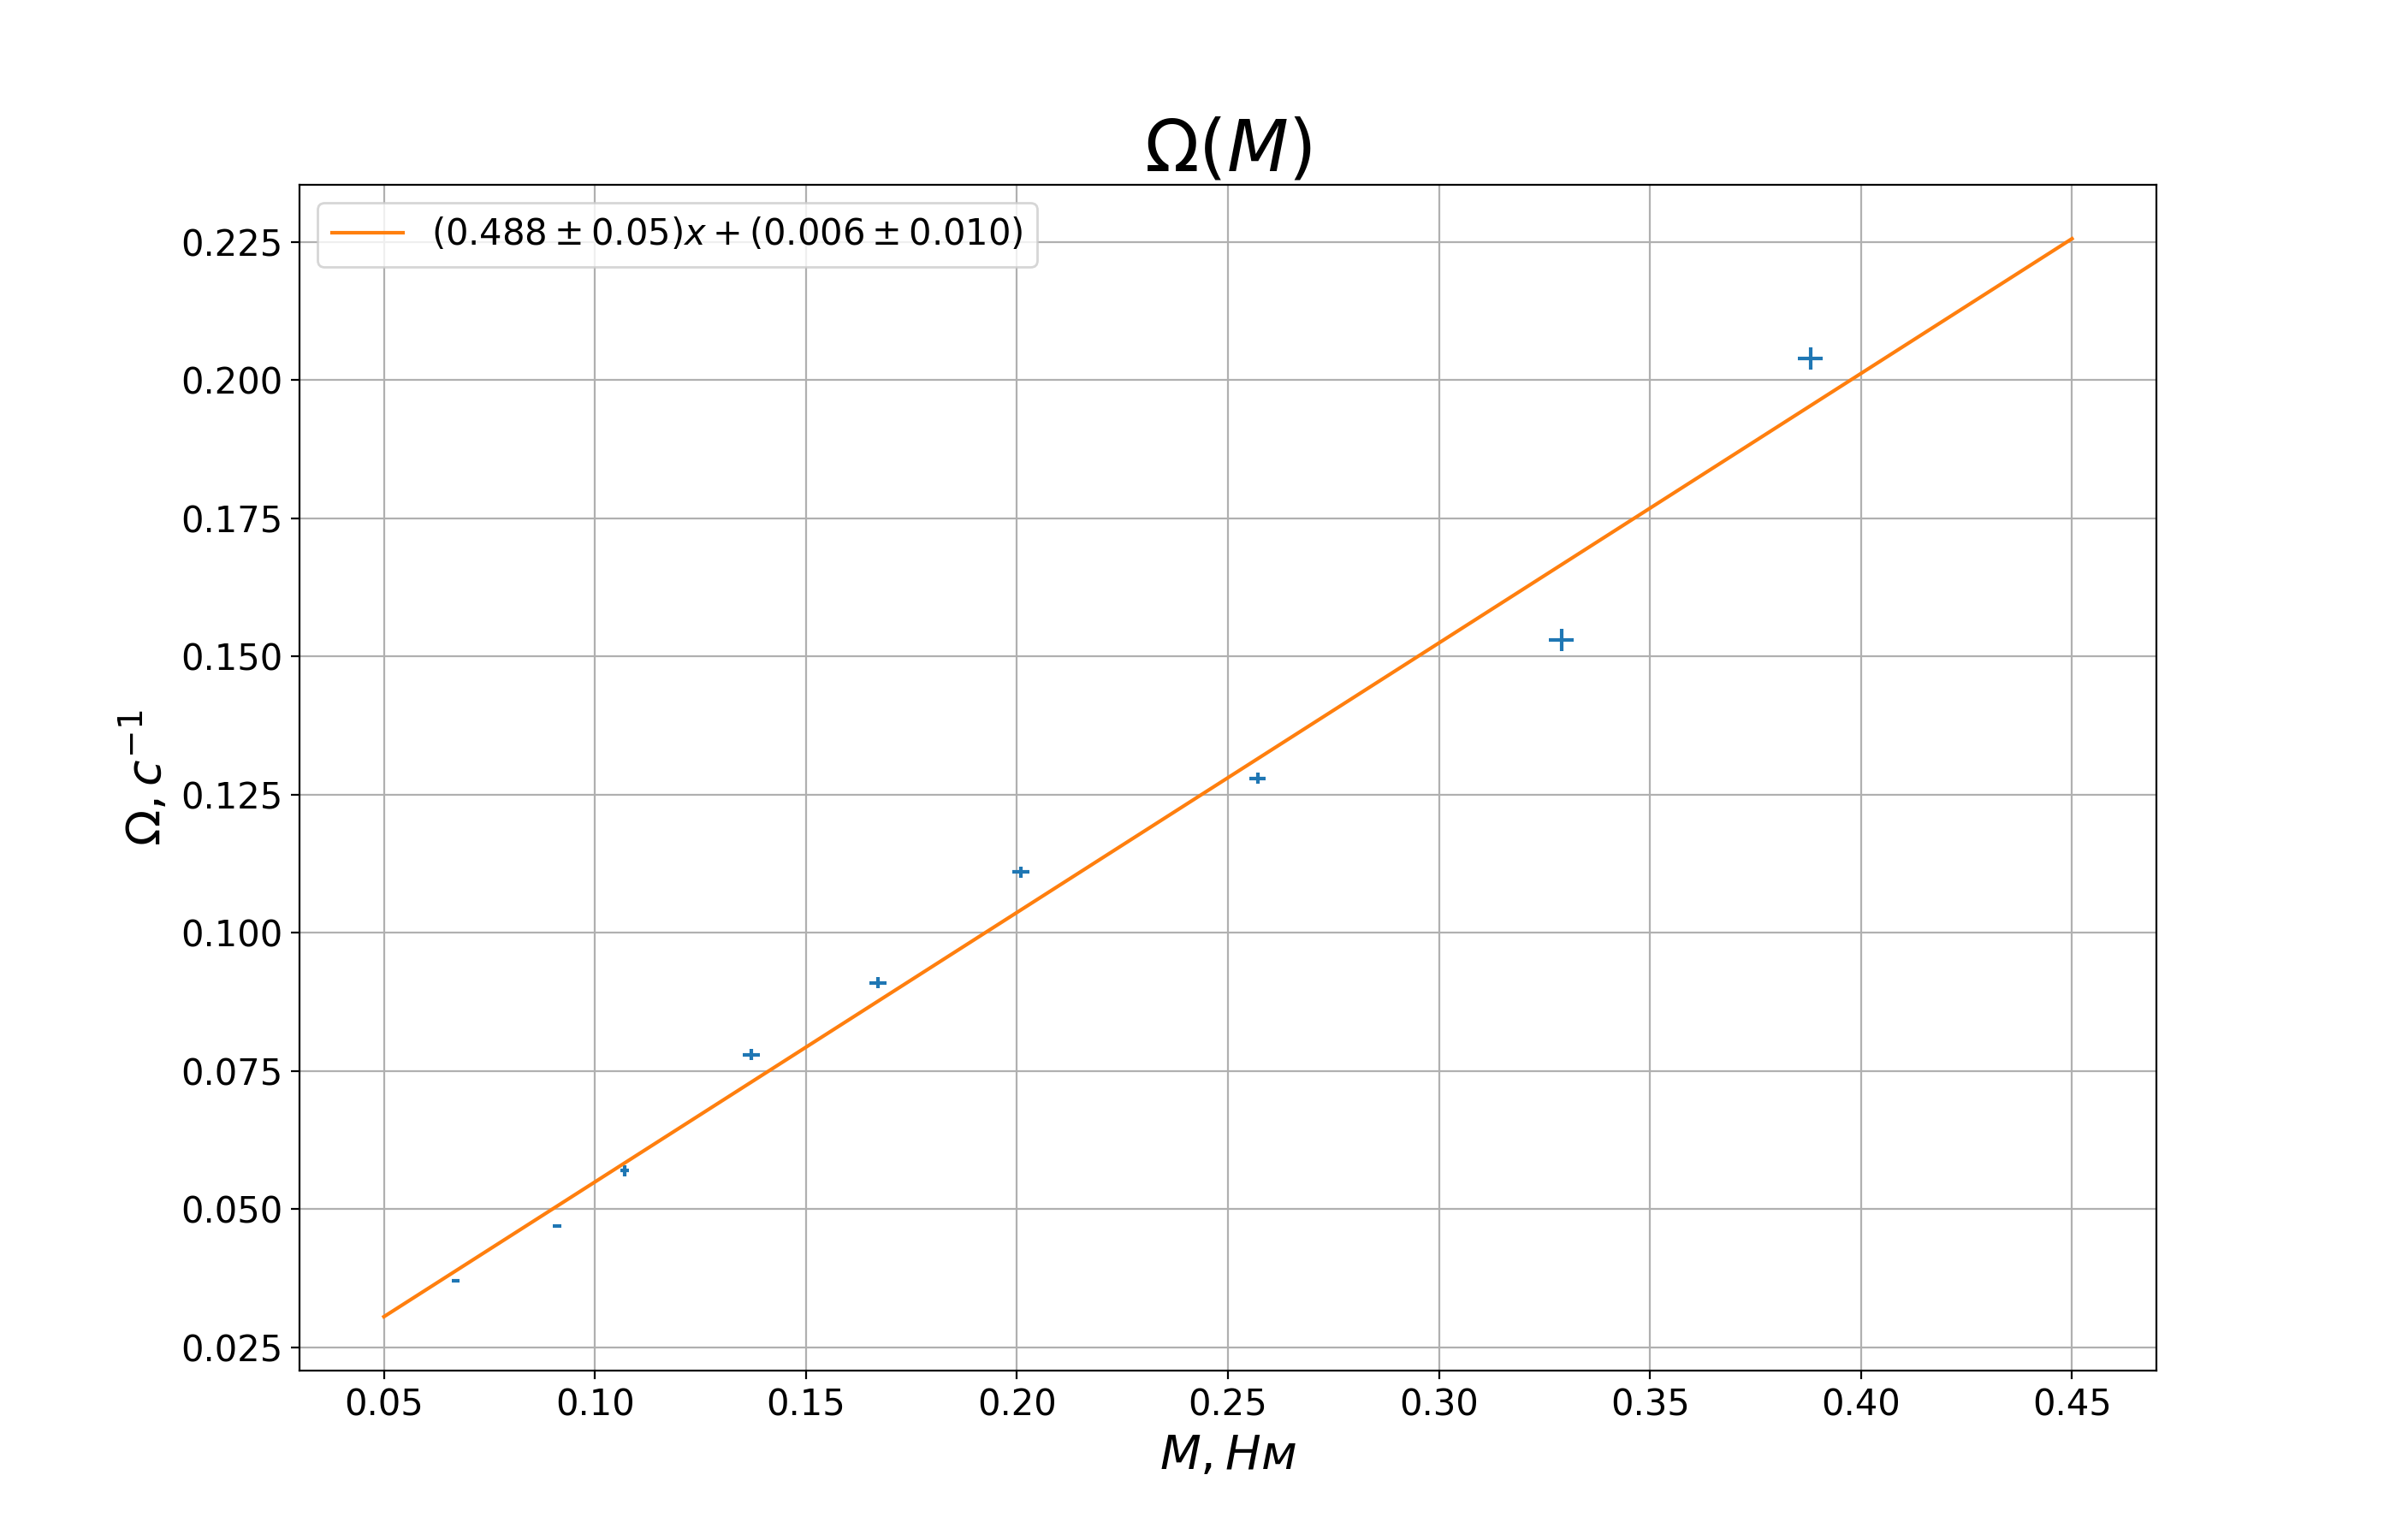
\includegraphics[width=0.7\textwidth]{img/plot.png}
    \caption{Графики зависимости для метода саморепродукции}
    \label{fig:plot}
\end{figure}

\subsection{Результаты измерения решеток}
Сводка результатов измерений в таблице ниже. 

\begin{table}[!ht]
    \centering
    \begin{tabular}{|l|l|l|l|l|l|}
    \hline
        Решетка & 1 & 2 & 3 & 4 & 5 \\ \hline
        Метод I & 0,020$\pm0,003$ & 0,034$\pm0,005$ & 0,060$\pm0,003$ & 0,114$\pm0,004$ & 0,159$\pm0,006$ \\ \hline
        Метод II & - & - & 0,089$\pm0,012$ & 0,140$\pm0,018$  & 0,153$\pm0,022$ \\ \hline
        Метод III & - & - & 0,093$\pm0,011$ & 0,136$\pm0,016$ & 0,170$\pm0,035$ \\ \hline
    \end{tabular}
\end{table}

Можно заметить, что наиболее крупная решетка имеет наиболее близкие друг к другу результаты, в то время, как значения для остальных отличаются при вычислении разными методами. Численная погрешность меньше всего при измерениях первым методом. Отметим, что первый метод также оказался единственным, применимым для измерения периодов мелких решеток.

\subsection{Исследование миры}
В установку предыдущего пункта вместо кассеты с решетками вставлена мира. Аналогичным образом, тремя методами измерены параметры решетки №25, затем №20. Поскольку все вычисления совершенно аналогичны предыдущим пунктам, приведём лишь результаты.

\begin{table}[!h]
    \centering
    \begin{tabular}{|l|l|l|}
    \hline
        Решётка миры & №20. d, см & №25. d, см \\ \hline
        Метод I & 0,039$\pm0,004$ & 0,051$\pm0,005$ \\ \hline
        Метод II & 0,049$\pm0,008$ & 0,063$\pm0,012$ \\ \hline
        Метод III & 0,089$\pm0,013$ & 0,117$\pm0,017$ \\ \hline
    \end{tabular}
\end{table}

Заметим, что результаты последнего метода сильнее всего отличаются от остальных. Погрешность измерений так же, как и в опытах с решёткам, оказалась наименьшей при измерении параметров простраственного спектра. 

\section{Выводы}
В работе мы изучили саморепродукцию и применили его к измерению периодов дифракционных решеток. Параметры данных периодических структур измерены двумя дополнительными методами (по спектру и по увеличенному изображению через линзу). Дополнительные методы измерения дали совпадающие по порядку результаты, однако сходятся сточностью до коэффициента с остальными методами. Результаты измерений и их сравнение представлены в таблицах выше. 

Явления саморепродукции позволило довольно точно оценить параметры решёток по порядку величины, однако наиболее результативным оказался метод измерения пространственного спектра.

\end{document}
%все